\begin{document}
\section{TradingBot}
%% Vorwort
Im heutigen Zeitalter möchten Menschen so wenig Arbeit wie möglich aufwenden, dennoch aber die bestmöglichen Gewinne erzielen. Hier greift der TradingBot. Viele verbinden mit dieser Software automatisches Geld verdienen ohne viel Zeit zu vergeuden. Im Folgenden Kapitel werden die Vor- und Nachteile des Bots aufgezeigt und wie die Software hier zum Einsatz kommt. 
%% Ende Vorwort

%% Recherche
\subsection{Recherche}
Die Crypto Projektgruppe der Universität Oldenburg hat bereits ein ähnliches Programm entwickelt und eine Dokumentation veröffentlicht. Mithilfe dieser Informationen konnten Punkte eingebracht werden, die Anfangs weniger Beachtung erhalten hätten.\cite{deepCrypto}
%% Ende Recherche

%% Ziel
\subsection{Ziel}
Ziel ist es, dass eine automatisierte Abwicklung von Trades stattfindet, so dass der Nutzer eine Hilfe beim Handeln mit z. B. Kryptowährungen hat. Die Absicht der Verwendung einer solchen Software ist, die menschlichen Eigenschaften wie Angst, Gier und Risiko außen vor zu lassen. Jeder Mensch wird von diesen Punkten gesteuert und kann somit beim Traden zu früh oder auch zu spät Entscheidungen treffen. Ein solches Programm kann hierbei helfen, indem der Verwender keine Trades vorzeitig beenden kann, wenn diese über die Software gesetzt wurden.
\begin{figure}[ht]
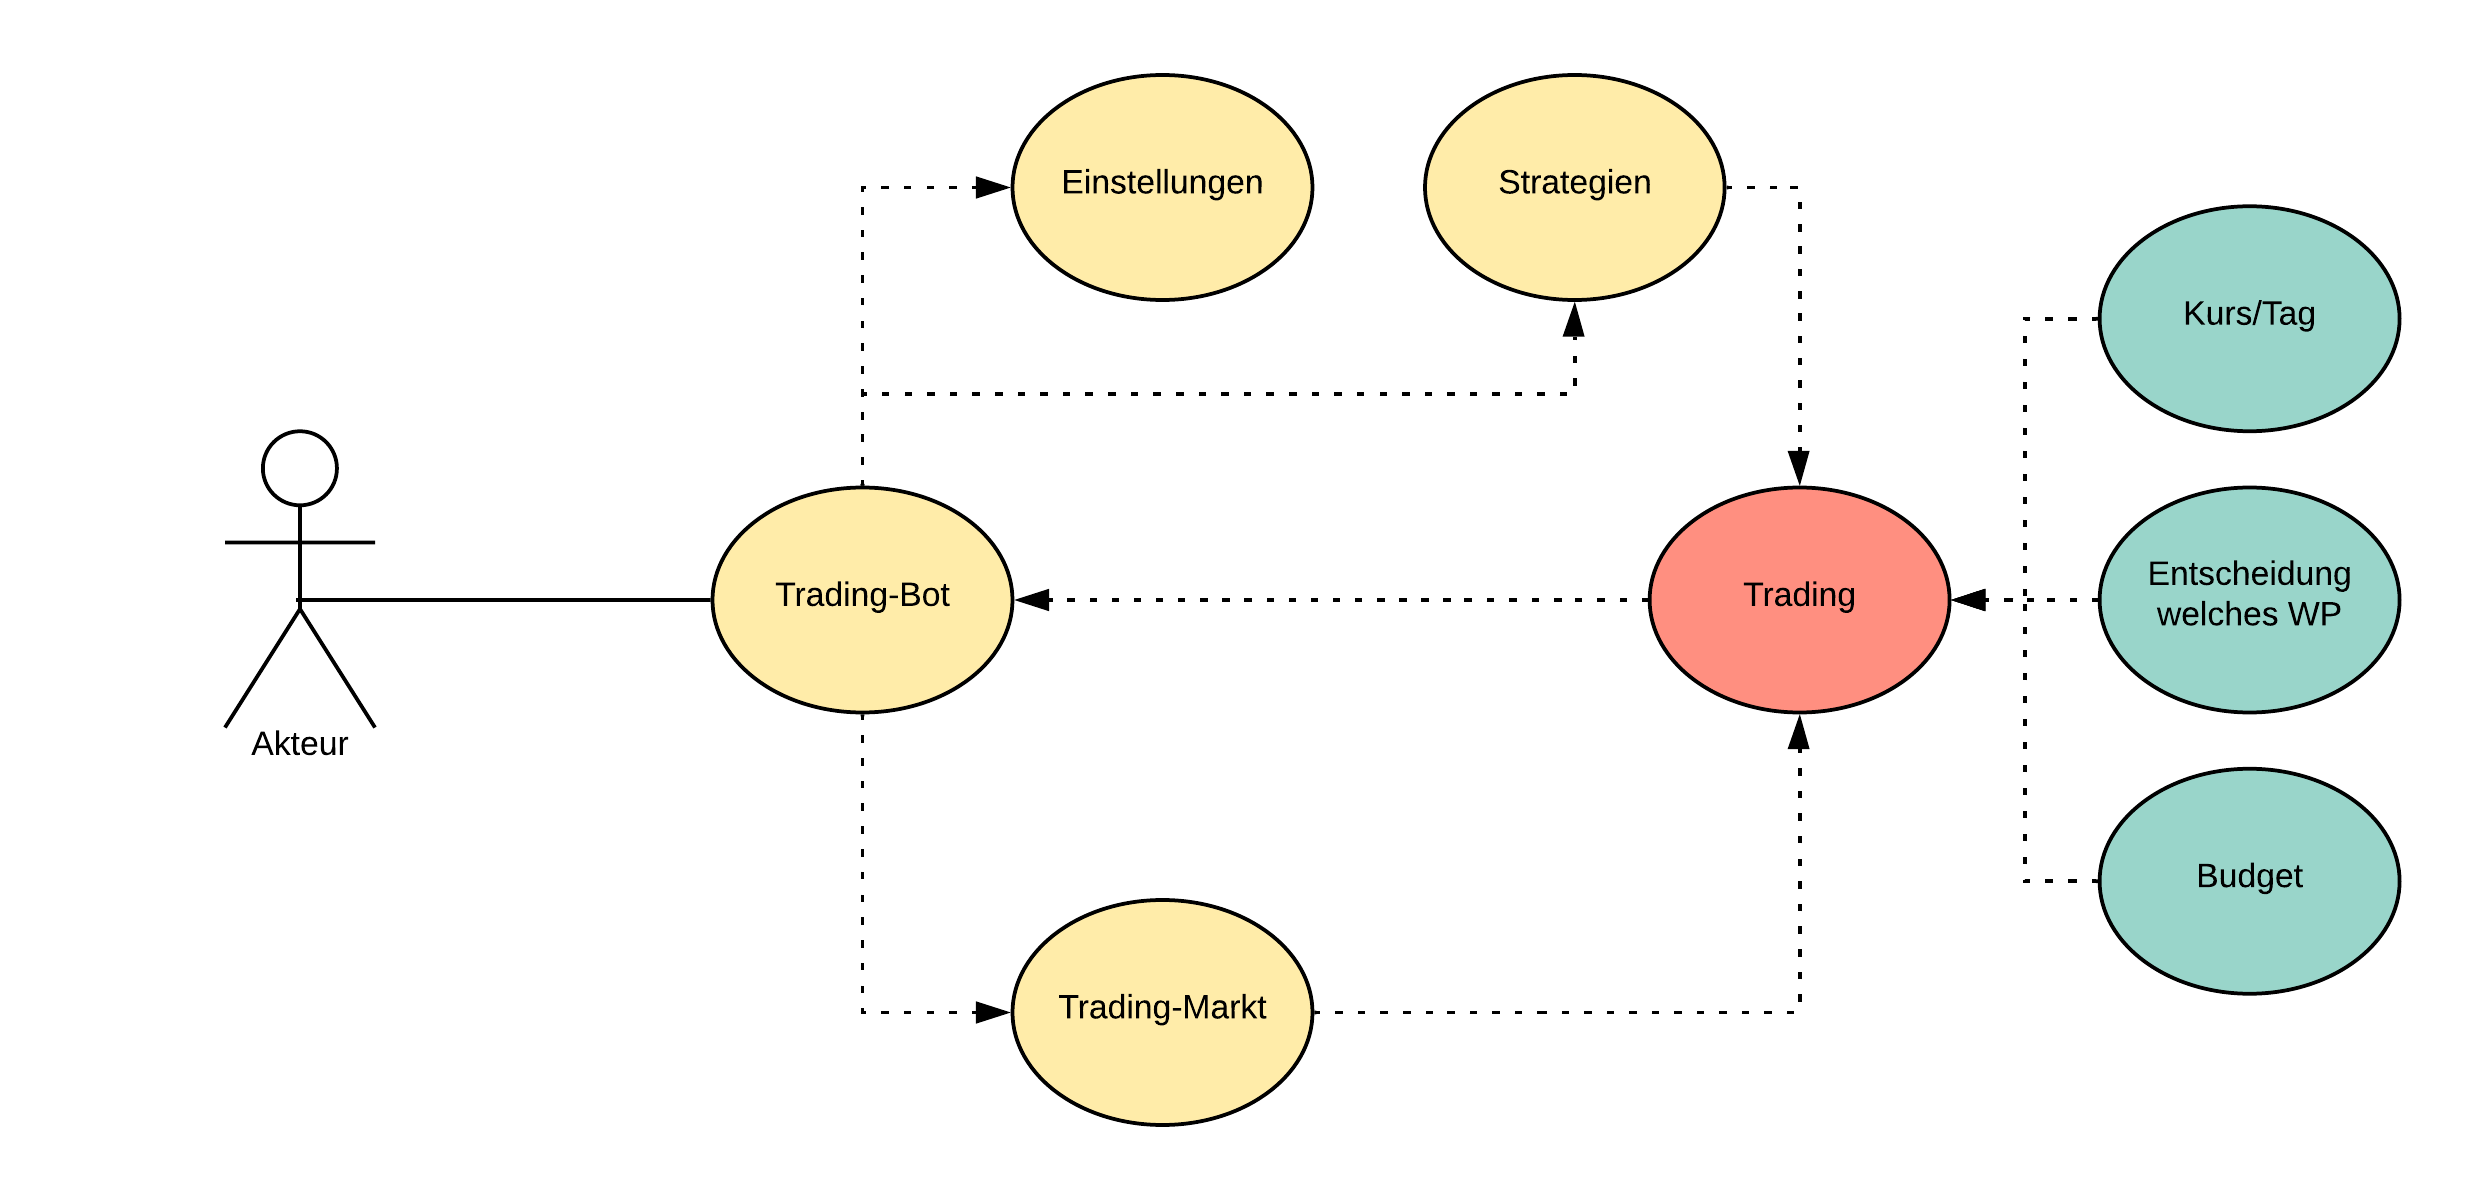
\includegraphics[width=5cm]{bot/trading_diagramm}
\caption{Trading Ablauf}
\label{Trading_Diagramm}
\end{figure}
%% Ende Ziel

%% Schnittstelle
\subsection{Schnittstelle}
Dieser TradingBot soll eine Schnittstelle zu einem Dashboard bieten. Aktuell läuft die Software nur in der Console und kann nicht verändert werden.
\begin{figure}[ht]
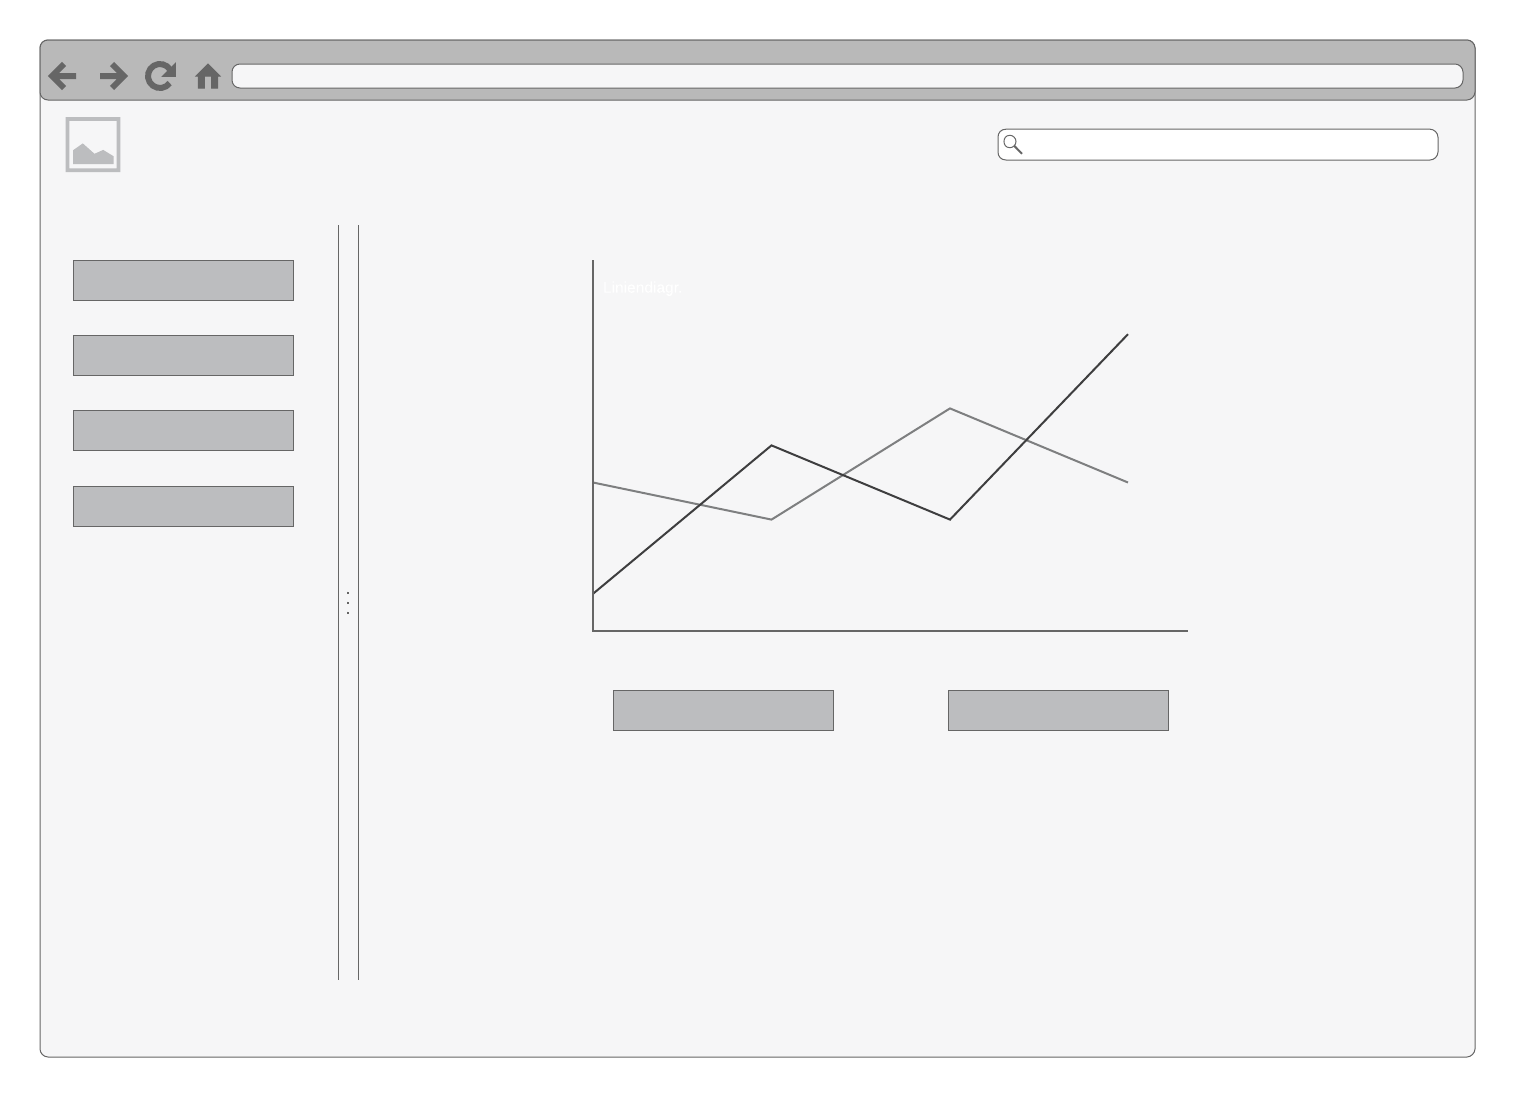
\includegraphics[width=5cm]{bot/wireframe_bot}
\caption{Wireframe Dashboard}
\label{Wireframe_Dashboard}
\end{figure}
\\
Sobald die Funktionalität ausgereift ist und genügend ausgewertete Daten zur Verfügung stehen, können die Ausarbeitung und das Implementieren in eine graphische Oberfläche begonnen werden.
%% Ende Schnittstelle

%% Funktionalität
\subsection{Funktionalität}
Der TradingBot erhält unterschiedliche Clients, die alle Aufgaben abarbeiten. Nachfolgend werden die Funktionalitäten dieser Clients aufgeführt.
\begin{figure}[ht]
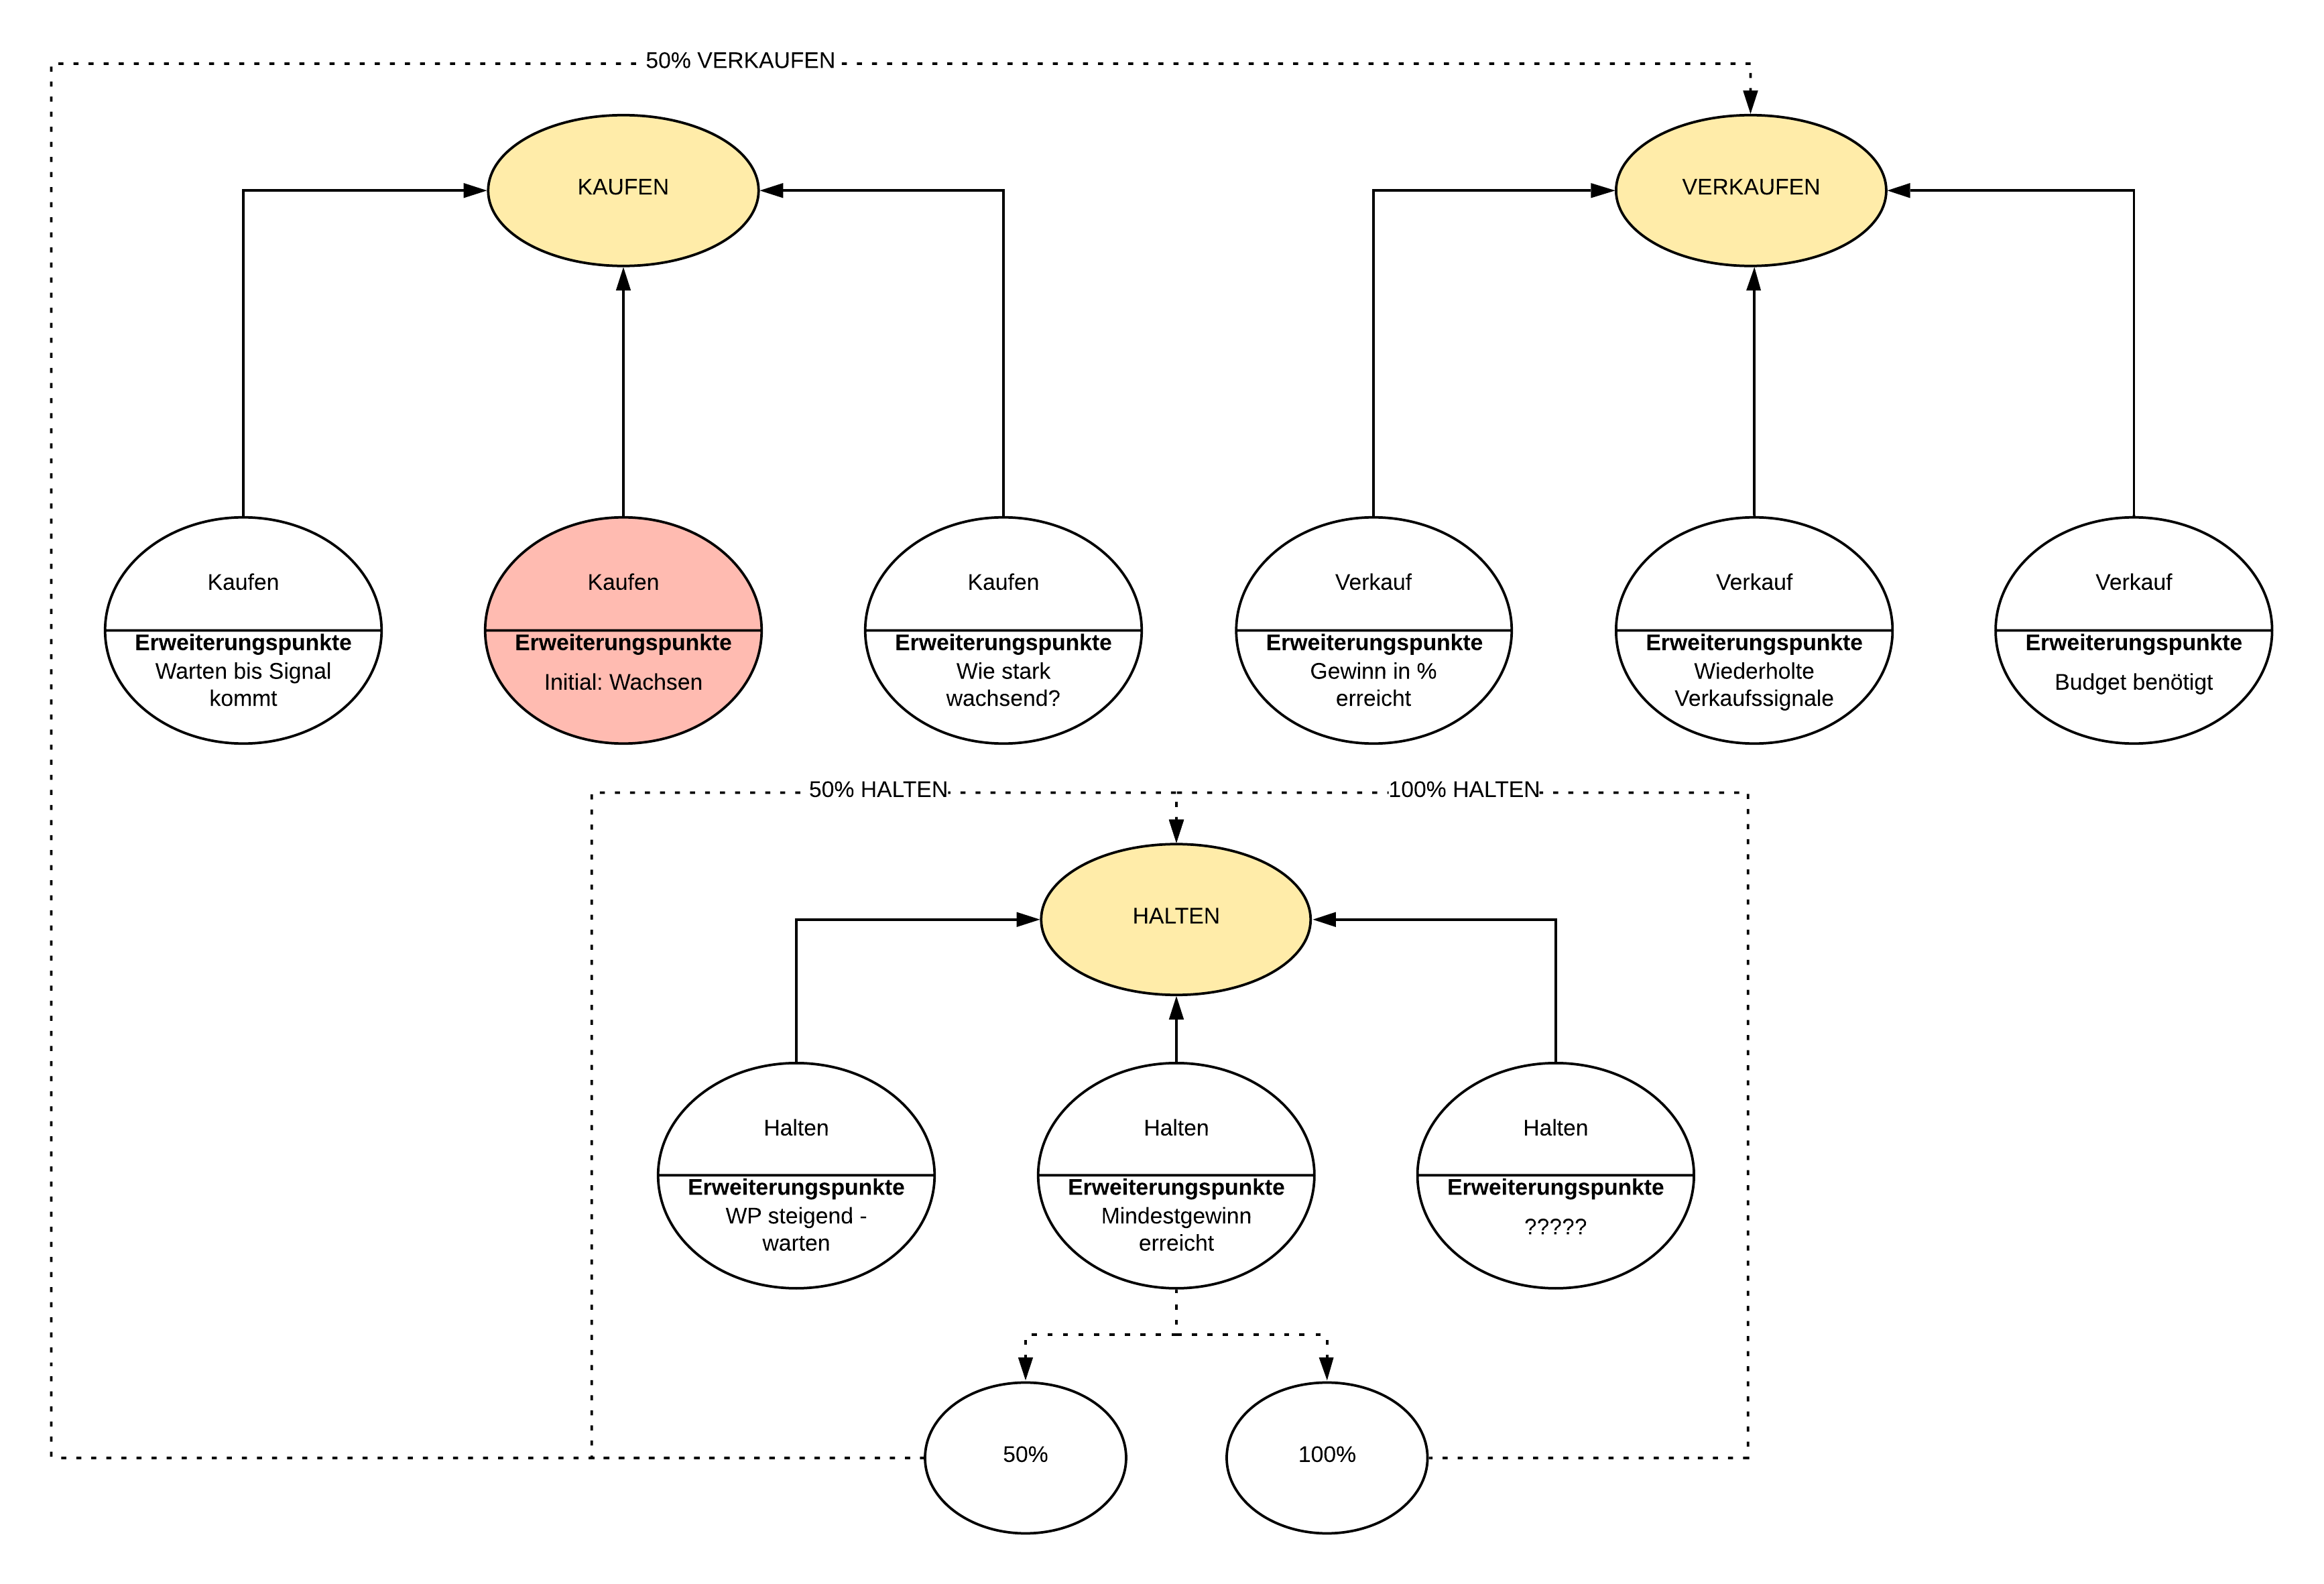
\includegraphics[width=5cm]{bot/funktionen_diagramm}
\caption{Funktionalität Diagramm}
\label{Funktionalität_Diagramm}
\end{figure}
\\
\subsubsection{Persistenz}
Um die Tätigkeiten der Software zu kontrollieren, werden alle durchgeführten Aktionen geloggt. Hierfür wird der Persistenz-Client benötigt, so dass alle Daten gespeichert und aufgerufen werden können, wenn ein Nutzer diese einsehen möchte.
\subsubsection{API-Schnittstelle}
Aktuell wird hier eine Schnittstelle künstlich erzeugt, die lediglich ausgibt, bestimmte Aktionen durchzuführen. Hier werden Schnittstellen zu Handelsplattformen eingepflegt um im Live-Modus effektiv zu handeln.
\subsubsection{Portfolio}
Jeder aktive Trader hat ein Portfolio, welches alle Angebote beinhaltet. Hier kann der Bot einsehen, welche dieser Trades bearbeitet werden müssen, falls ein Signal dafür erscheint.
\subsubsection{Guthaben}
Da ein Trade nur gesetzt werden kann, wenn das nötige Budget auf dem Nutzerkonto vorhanden ist, wird mit einem Budget-Client dieses überwacht. Jede Transaktion passt das Guthaben automatisch an.
\subsubsection{Kaufen}
Um einen Trade zu setzen wird ein Buy-Helper verwendet. Dieser bekommt die Schnittstelle und das Signal übergeben. So kann der Bot auf der richtigen Handelsplattform arbeiten. Jedes Signal hat eine Stärke, diese bestimmt dann die Kaufkraft. Aktuell werden pro Trade maximal 10\% des Guthabens verwendet. 
\begin{figure}[ht]
\begin{lstlisting}[language=Python]
if (strength == '0'):
 self.signal_amount = 0.15
elif (strength == '1'):
 self.signal_amount = 0.33
elif (strength == '2'):
 self.signal_amount = 0.66
elif (strength == '3'):
 self.signal_amount = 1.0
\end{lstlisting}
\caption{Bestimmung der Höhe einer Buy-Order}
\end{figure}
\\Mit dem Signal-Objekt wird eine Offer erzeugt, diese wird dann an den API-Client übergeben und der Trade wird gesetzt.
\subsubsection{Verkaufen}
Ähnlich wie das Kaufen wird auch der Verkauf durchgeführt. Der Sell-Helper wird mit der API und dem Signal aufgerufen und dadurch wird eine Offer erstellt. Ist dies erledigt, wird die Offer an die API übergeben und der Trade mit einer Restsumme neu gesetzt oder aber geschlossen.
%% Ende Funktionalität

%% Vor- und Nachteile
\subsection{Vor- und Nachteile}
Nachfolgend werden die Vor- und Nachteile eines Bots erklärt.
\subsubsection{Vorteile}
Durch den Einsatz einer Software für das Handeln mit Währungen können Emotionen minimiert werden, so dass es nicht zu einem voreiligen Verkauf kommt. Des weiteren hält sich der Bot mit hoher Disziplin an die Vorgaben. So werden keine höheren Profite erzwungen, die oft zu einem Verlust führen können. Der Bot wird mit den Regeln für das Handeln getestet, in dem historische Daten verwendet werden.
\subsubsection{Nachteile}
Jedoch können Programme auch Fehler aufweisen. Somit kann es passieren, dass aufgrund von Internetproblemen ein Trade nicht abgeschlossen werden kann. Weil diese Software TradingBot heißt, bedeutet dies jedoch nicht, dass alles selbständig abläuft. Eine Software muss immer kontrolliert werden um Fehlverhalten feststellen zu können.
%% Ende Vor- und Nachteile

%% Stand
\subsection{Stand}
Der aktuelle Stand ist, dass die Software an einem beliebigen Tag startet und von dort ab 30 Tage handelt. Jeder Tag wird lokal festgehalten und wird somit kontrollierbar. Aufgrund fehlender Daten, konnten nur künstlich erzeugte Daten zum Testen verwendet werden. Hier ist es nun wichtig, dass ein weiterer großer Test mit Echtzeit-Daten stattfindet, um den Effekt der hier genannten Indikatoren und Strategien zu testen. 
%% Ende Stand
\end{document}